% Document class options: % ======================= %
% serif: Sets the body font to be serif.
%
% twocolumn: Sets the body text in two - column layout.
%
% Fill in the type of article here.
% empirical % reflection % meta % rga % editorial %
% Using other bibliography styles: % ======================= % authordate = APA % number =[1] %
 \documentclass[twocolumn, serif, empirical, authordate]{jote-article}
 %%% Add the bibliography, make sure it's in the same directory
\addbibresource{hartman.bib}
 %%% Add additional packages here if required.Usually not needed, except when doing things with figures and tables, god help you then % This package is for generating Lorem Ipsum, usage: \lipsum[X] where X is the Xth paragraph of lorem ipsum.OR use[1 - 5] to generate the first five, etc.nnn

\usepackage{balance}
\usepackage{gensymb}
\usepackage{graphicx}
\usepackage[export]{adjustbox}% http://ctan.org/pkg/adjustbox %%% TODO: Make this a 1 - 5 option scale to reduce the chance of mistyping % Enter the title, in Title Case Plennnnnnnnnnnnnnase % Try to keep it under 3 lines
 \title{The Gloria Adherence Subproject: Problems and Randomization Mistakes}
 % List abbreviations here, if any.Please note that it is preferred that abbreviations be defined at the first instance they appear in the text, rather than creating an abbreviations list.
%\abbrevs{ % ABC, a black cat; DEF, doesn't ever fret; GHI, goes home immediately.}
 % Include full author names and degrees, when required by the journal.
% Use the \authfn to add symbols for additional footnotes and present addresses, if any.Usually start with 1 for notes about author contributions; then continuing with 2 etc if any author has a different present address.
% Format: \author[1, 2]{FirstName LastName} \author[2]{...}

\author[1, 2]{Linda~Hartman}
\author[3]{Marc~R.~Kok}
\author[4]{Esmeralda~Molenaar}
\author[5]{Ed~N.~Griep}
\author[6]{Jaap~M.~Van~Laar}
\author[7]{Jan~Maarten~Van~Woerkom}
\author[8]{Cornelia~F.~Allaart}
\author[9]{Hennie~G.~Raterman}
\author[10]{Yvonne~P. M.~Ruiterman}
\author[11]{Marieke~J. H.~Voshaar}
\author[12]{Jo\~ao~Redol}
\author[13]{Rui~M.~A.~Pinto}
\author[2]{L.~Thomas~Klausch}
\author[1]{Willem~F.~Lems}
\author[1, 2]{Maarten~Boers}

 % Fill it in again for the PDF metadata.Lame workaround but it works % Format: \authorone{...} \authortwo{...}
 \authorone{Hartman et al.}
 % List the contribution effort here, they will be listed at the end of the page % List the acknowledgments.If there is no companion piece, this is listed below the author info %
 %\acknowledgments{
 %J. W. J. Bijlsma, R. Christensen, Y. M. Smulders and S. H. Ralston are members of the scientific advisory committee of the GLORIA trial.
%}
% List possible conflict of interest.Will default to saying no conflict exists.
%\interests{Author One was paid for by Big Failed Experiment}
% List funding %
% \funding{ The GLORIA project was funded by the \emph{European Union's Horizon 2020 Research and Innovation Programme} under the topic `Personalizing Health and Care' (grant number 634886).}
% Include full affiliation details for all authors

\affil[1]{Amsterdam Rheumatology and Immunology Center, Amsterdam UMC, location VUmc, Amsterdam, Netherlands}
\affil[2]{Epidemiology \& Data Science, Amsterdam UMC, Vrije Universiteit, Amsterdam, Netherlands} \affil[3]{Department of Rheumatology and Clinical immunology, Maasstad Hospital, Rotterdam, Netherlands} \affil[4]{ Department of Rheumatology, Groene Hart Hospital, Gouda, Netherlands} \affil[5]{Department of Rheumatology, Antonius Hospital, Sneek, Netherlands}
\affil[6]{Department of Rheumatology and Clinical Immunology, University Medical Center Utrecht, Utrecht, Netherlands}
\affil[7]{Department of Rheumatology, Gelre Hospitals, Apeldoorn, Netherlands} \affil[8]{Department of Rheumatology, Leids University Medical Center, Leiden, Netherlands}
\affil[9]{Department of Rheumatology, Northwest Clinics, Alkmaar, Netherlands} \affil[10]{Department of Rheumatology, Haga Hospital, Den Haag, Netherlands} \affil[11]{Tools Patient Empowerment, Amsterdam, Netherlands} \affil[12]{BeyonDevices LDA, Sobral de Monte Agra\c{c}o, Portugal} \affil[13]{Bluepharma, Ind\'ustria Farmac\^eutica, S.A., Coimbra, Portugal}
% List the correspondence email of the main correspondent
\corraddress{Linda Hartman  \href{l.hartman@amsterdamumc.nl}{l.hartman@amsterdamumc.nl}}
 % Optionally list the present address of one of the authors %\presentadd[\authfn{2}]{Department, Institution, City, State or Province, Postal Code, Country}
 % Fill in the DOI of the paper % Always starts with '10.36850/' and is suffixed with one of the following plus a number % e : empirical % r : reflection % mr : meta - research % rga: rejected grant application % ed : editorial \paperdoi{10.36850/TOBEFILLEDIN}
 % Include the name of the author that should appear in the running header
 \runningauthor{Hartman et al.}
 % The name of the Journal
 \jname{Journal of Trial and Error}
 % The year that the article is published
 \jyear{2021}
 % The Volume Number
 % \jvolume{Fall}
 % The website that's listed in the bottom right \jwebsite{ https://www.jtrialerror.com}
 %%% Only \paperpublished is necessary, any combination of the other two is possible % When the paper was received % Format: 1 January, 1900
 \paperreceived{3 June, 2021}
 % When the paper was accepted % Format: 1 January, 1900
 \paperaccepted{24 August, 2021}
 % When the paper will be published % Format: 1 January, 1900
 \paperpublished{18 October, 2021}
 % When the paper is published but in YYYY - MM - DD format, for the crossmark button
 \paperpublisheddate{2021-10-18}
 % The pages of the article, comment out if rolling article
 % \jpages{1 - 12}
 % Link to the logo, might be redundant
 \jlogo{media/jote_logo_full.png}
 % Fill something here if this is a rolling / online first article, will make ROLLING ARTICLE show up on the first page \rolling{}
 % Sets the paragraph skip to be zero, this should be in the CLS
 \setlength{\parskip}{0pt}
 %%% Companion Piece % Reflection and Empirical articles have each other as companion pieces.Add the DOI, Title, and Abstract of the respective Companion piece here %%% Abstract % These two set the height and width of the abstract.There's no solution to do this automatically at the moment so fiddle with these a bit. height-width should be 5mm, and ranges between 50-100 are realistic % Higher number means skinnier abstract
 \heightabstract{70mm}
 \widthaffil{65mm}
% Enter something here in order for the abstract to disappear.Be sure to also delete the abstract \noabstract{}
% Fill in the keywords that will appear in the abstract, max 7
 \keywordsabstract{
 medication adherence, electronic caps, rheumatoid arthritis, nested trial, randomization
 }

 %%%%%%%%%%%%%%%%%%%%%%%%%%%%%%%%%%%%%%%%%%%%%%%%%%%
% Document Starts %%%%%%%%%%%%%%%%%%%%%%%%%%%%%%%%%%%%%%%%%%%%%%%%%%%
 \begin{document}
 %%% This starts the frontmatter, which includes everything that's on the front page execpt the text of the article
 \begin{frontmatter}
   \maketitle % Type your abstract between these things.Max 250 words.Be sure to include the \noindent, looks bad otherwise
   \begin{abstract}
  Medication adherence, which is the extent to which patients take their medication as prescribed, is essential in treating chronic inflammatory diseases such as rheumatoid arthritis (RA). Therefore, we nested a subproject in the two-year multicenter Glucocorticoid Low-dose Outcome in Rheumatoid Arthritis (GLORIA) trial to add a low-dose prednisolone (5 mg/day) or placebo to the standard care in older people (65+ years) with RA. Adherence was measured with an electronic monitoring cap that recorded bottle openings in all patients. In the subproject, we performed an adherence intervention with an advanced cap that could communicate with an application on the smart device via Bluetooth. We randomized patients with a smart device to receive or not to receive adherence reminders on the smart device for three months. Multiple problems emerged that precluded an answer to the research question: sample size (overly optimistic estimates of older patients with a smart device), logistic issues (availability of smartcaps, data extraction), randomization and treatment allocation errors (despite training of personnel), and low quality of the data in the intervention group (hardware failure, discovered too late because data was read in batches). For future trials planning to include a subproject, we recommend keeping it simple, starting with a field test before the actual study starts, and monitoring data from the beginning of the study. \end{abstract}
 \end{frontmatter}
 




\section*{Take home message}
 It proved difficult to perform a subproject nested within a large investigator-initiated trial, although we expected it to be easy. We recommend keeping a nested subproject simple, maintaining active contact with study centers, and monitoring data from the beginning to resolve emerging problems immediately.



\section*{Purpose}

 The ongoing two-year Glucocorticoid Low-dose Outcome in Rheumatoid Arthritis (GLORIA) trial examines the addition of daily low-dose (5 mg)
prednisolone or placebo to the standard care in elderly patients (65+ years) with rheumatoid arthritis; adherence is measured with electronic caps and counting returned pills. A subproject was nested within the main GLORIA trial, limited to patients with a smart device who had taken the study treatment for at least three months. The objective was to test the effectiveness of adherence reminders delivered to the smart device through Bluetooth by a special cap during a three-month period. Eligible patients were randomized to the intervention group (receiving reminders)
or the control group (no reminders). In the intervention group, an application was loaded onto the smart device that communicated with the adherence-monitoring device loaded into the cap of the drug bottle. The app sent a reminder message if the patient had forgotten to take the study medication. The hypothesis was that after three months, patients in the intervention group would be more adherent compared to the patients in the control group. Multiple problems prevented us from answering our research question. This paper reflects on these problems.
The research group was a part of the GLORIA consortium and was comprised of rheumatologists and researchers from the Netherlands, Germany, Italy, and Portugal, and the owner of the caps and the pharmaceutical manufacturer of the study medication from Portugal.


\section*{Introduction}

 Medication adherence, which is the extent to which patients take their medication as prescribed (\pdftooltip{{\color{tip}Brown \& Bussell,}}{Brown, M. T., \& Bussell, J. K. (2011). Medication adherence: WHO cares? Mayo Clinical Proceedings, 86(4), 304–314.} \citeyear{Brown2011}), is essential to treat chronic inflammatory diseases, such as rheumatoid arthritis (RA; \pdftooltip{{\color{tip}Jungst et al.,}}{Jungst, C., Graber, S., Simons, S., Wedemeyer, H., \& Lammert, F. (2019). Medication adherence among patients with chronic diseases: A survey-based study in pharmacies. QJM: An International Journal of Medicine, 112(7), 505–512.}~\citeyear{Jungst2019}). Almost half of patients with chronic diseases are non-adherent (\pdftooltip{{\color{tip}Jungst et al.,}}{Jungst, C., Graber, S., Simons, S., Wedemeyer, H., \& Lammert, F. (2019). Medication adherence among patients with chronic diseases: A survey-based study in pharmacies. QJM: An International Journal of Medicine, 112(7), 505–512.}~\citeyear{Jungst2019}; \pdftooltip{{\color{tip}Kini}}{Kini, V., \& Ho, P. M. (2018). Interventions to improve medication adherence: A review. The Journal of the American Medical Association, 320(23), 2461–2473.}, \citeyear{Kini2018}). Non-adherence substantially increases the risk of a disease flare in RA (\pdftooltip{{\color{tip}Jungst et al.,}}{Jungst, C., Graber, S., Simons, S., Wedemeyer, H., \& Lammert, F. (2019). Medication adherence among patients with chronic diseases: A survey-based study in pharmacies. QJM: An International Journal of Medicine, 112(7), 505–512.} \citeyear{Jungst2019}).
 In the two-year multicenter Glucocorticoid Low-dose Outcome in Rheumatoid Arthritis (GLORIA) trial, a low-dose prednisolone (5 mg/day)
or placebo was added to the standard care in older people (65+ years)
with RA. We measured adherence with electronic monitoring and pill count in all patients (\pdftooltip{{\color{tip}Hartman et al.,}}{Hartman, L., Cutolo, M., Bos, R., Opris-Belinski, D., Kok, M. R., Griep-Wentink, H., Klaasen, R., Allaart, C. F., Bruyn, G. A. W., Raterman, H. G., Voshaar, M. J. H., Gomes, N., Pinto, R. M. A., Klausch, L. T., Lems, W. F., \& Boers, M. (2021). Medication adherence in older people with rheumatoid arthritis is lower according to electronic monitoring than according to pill count. Rheumatology.} \citeyear{Hartman2021}). In a subproject nested within the trial, we assessed the efficacy of an adherence intervention for the patients with a smart device.


\section*{Methods}

 The eligibility criteria for the subproject were to: be in possession of a smart device (smartphone or tablet) and be an active participant in the main GLORIA trial for at least three months. We planned to include patients with a smart device from all seven participating countries of the main trial because a pilot survey indicated that a sufficient number of patients (20\%) possessed a smart device in all countries. Based on this feasibility assessment, we expected to include 50 patients.
 Before the training of the study personnel, it appeared that only Dutch patients had smart devices. Therefore, the training of the study personnel was only provided in the Netherlands.


\subsection*{Training of study personnel}

 The study personnel of all participating Dutch sites received an e-mail with information about the objective of the subproject, eligibility criteria, signing of the informed consent in duplicate, and an explanation about the randomization step. In addition, the study personnel received a manual that explained the subproject procedures (assembling of the cap, installation of application) that were needed before the patient could start with the subproject. Finally, the subproject and the related procedures were explained and demonstrated during the Dutch GLORIA researchers meeting, and an English instructional movie was sent to all participating centers. One of us (LH) served as the contact person for questions about the subproject.


\subsection*{Subproject procedure}

 Eligible patients were informed about the subproject by the research nurse and were asked to participate. Patients who provided written informed consent were randomly assigned to either the intervention or control group through the electronic case record form (eCRF). All patients continued taking the study medication (one pill per day) from the pill bottle as in the main trial. The opening and closing events of the pill bottle (to measure adherence) were registered by the electronic cap for all patients. Patients in the control group continued their participation in the main study without changes. For patients in the intervention group, several actions of the study personnel were needed.
 The instructions given to study personnel were as follows: 
\begin{enumerate}
\def\labelenumi{\arabic{enumi}.}
\item Assembling of smart adherence cap: \begin{enumerate}
 \def\labelenumii{\alph{enumii}.}
 \item Remove the regular cap from the medication bottle.
 \item Close the pill bottle with the plastic replacement cap.
 \item Write the kit number of the medication bottle on a label and stick the label inside the smart adherence cap.
 \item Remove the cover of the double-tape on the interior of the smart adherence cap.
 \item Assemble the smart adherence cap over the plastic replacement cap on the medication bottle, correctly aligned, and press it until you reach resistance. Keep it under pressure for at least 3 seconds.
 \end{enumerate}
\item Installation of the GLORIA app on the smart device of the patient: \begin{enumerate}
 \def\labelenumii{\alph{enumii}.}
 \item Open the Google Play store (Android)/App Store (iOS) application \item Search for "GLORIA adherence cap"
 \item Install the app and wait until the installation process has been finished \item Open the GLORIA application \end{enumerate}
\item Connecting the smart adherence cap and the GLORIA app via Bluetooth by going through multiple steps in the app. (see page 13-19 of appendix for the detailed instruction)
\end{enumerate}
 The activated app was connected to the smart adherence cap of the medication bottle via Bluetooth. For patients, no additional actions were required. The patient only had to open the medication bottle once per day, preferably in the morning. Both the regular adherence caps in the control group and the smart adherence caps in the intervention group recorded each opening and closing event of the medication bottle. The smart adherence cap repeatedly attempted to open a connection with the GLORIA app via Bluetooth to report whether the bottle had been opened.
If the bottle was not opened between 08:00 a.m. and 02:00 p.m., the app posted a notification on the opening screen to remind the patient to open the medication bottle. The patients in the control group did not receive an activated smart cap nor the reminder app; they were instructed to open the medication bottle once per day, as in the main trial. At the end of the three-month period, the bottle was returned, and the remaining capsules were counted. For patients that started the trial at six months or later, the return of the bottle was delayed by three months, because clinic visits occurred every six months. The adherence of both groups based on returned pills was calculated as follows: If the number of pills dispensed is D, the treatment period in number of days is P, and the number of pills returned is R, medication adherence (\%) is calculated as: ((D-R)/P)*100. The adherence of the two groups was compared.
 Social desirability could have influenced the adherence measurements with the caps and the number of returned pills. Patients might have returned the expected number of pills or opened the medication bottle as would be expected. However, we assume that most patients were as adherent as non-trial patients, because it would be difficult to maintain social desirability during the full two years of the trial.


\subsection*{Data registration and extraction}

 Apart from the bottle closing and opening events, which were always registered if the medication bottle was opened, the smart adherence caps also registered ``pairing success'' events, ``no communication'' events, ``keep alive'' events and ``reset'' events.
 The ``pairing success'' events guaranteed that the pairing of the adherence cap with the app before the study started was successful.
Non-registration of this event indicated that the pairing of the cap and app was unsuccessful and that the cap was not able to communicate with the smart device during the entire three months of the study (reported by ``no communication'' events). Therefore, caps with no ``pairing success'' event at the start of the study were excluded.


\subsection*{Opening events}

 ``No communication'' events were registered at 02:00 p.m. if the smart adherence cap had been unable to communicate with the app on the smart device between 08:00 a.m. and 02:00 p.m. on a given day. The time window from 08:00 a.m. until 02:00 p.m. was chosen to match the advice to take prednisolone in the morning. The registration of ``no communication'' events was independent of the successful or unsuccessful pairing between the app and the cap. The ``keep alive'' event was used to check if the cap still worked and if the battery was not empty. ``Keep alive'' events were registered one or more times per morning, indicating that the cap was functioning even if a patient did not open the medication bottle. A ``reset'' event was registered whenever a reset on the system was detected. This could be related to battery power being too low, or bad contacts on the battery power supply caused by faulty cables due to falls or abrupt movements of the cap. If more than one ``reset'' event was registered, the cap was excluded.
 The patients returned the regular caps and adherence caps to the research nurse, and the caps of each site were sent to the owner of the caps (BeyonDevices LDA, Sobral de Monte Agra\c{c}o, Portugal). The data of the caps were read in batches and were uploaded in data files. The data files contained the registration of the events described above. The app generated a reminder message if the cap did not transmit an opening event between 08:00 a.m. and 02:00 p.m., or if no communication was established on that day (registered in the cap).


\section*{Discussion}



\subsection*{Problems in the preparation and execution of the trial}

 We had multiple misfortunes related to the preparations of the subproject, technical issues with the app and smart adherence cap, and the randomization step. Therefore, it was not possible to test the effectiveness of adherence reminders delivered via the smart device during the three month trial period.
 We want to discuss and reflect on the problems and misfortunes that prevented us from answering our research question. All aspects that influenced the success of the subproject were discussed, and we reflected on how each aspect contributed to the subproject's failure.
 The discussions and reflections are mainly related to the researchers from the Netherlands, because only Dutch patients entered the subproject. The discussions were supported by the scientific advisory committee, which was set up especially for the GLORIA trial and by the developers of the adherence caps and the GLORIA app.


\subsection*{Preparations}

 We had a contract with a company that would deliver the adherence caps and the application for the subproject, but this company went bankrupt a few months before the study would start. We had to choose another company in a very short time frame because the main trial was almost ready to start. This choice was based on expertise, the projected time for development and implementation of the smart device reminder app, and an offer with limited costs because the budget of this investigator-initiated study was limited. Unfortunately, the chosen company needed more time than expected to develop suitable smart caps.
In total, this caused a delay of 1.5 years in the delivery of the smart caps.


\subsection*{Sample size}

 The number of potential patients for the subproject proved much lower than expected. From initial feasibility assessments among the trial centers, it appeared that around 20\% of the elderly patients possessed a smart device. Assuming that patients with a smart device are technically interested, we expected that about 80\% of them would be willing to participate. Thus, with a sample size of 450 patients in the main study, we expected around 72 patients in the subproject. As it turned out, smart device owners in this senior population were only located in the Netherlands. This resulted in a significant waste of paid and unpaid work hours: The app and instruction manual were translated from English into seven localized versions with the help of the patient panel of the main trial. To include enough patients in the subproject, we amended the protocol so that patients could start with the subproject at any moment during the trial instead of only at the three-months visit.


\subsection*{Complexities for the participating sites}

 The changed inclusion moment for the subproject (as described above)
made the inclusion procedure more complex for the participating sites.
 Another potential source of confusion was that we now had two types of similar-looking caps: the regular adherence caps used by all patients throughout the whole main trial, and the smart adherence caps only intended for patients in the intervention group of the subproject. The only difference between the caps was the color of the magnetic label on the cap, which had to be removed to activate the cap. It proved difficult for the research nurses to remember the differences and objectives of the regular and smart adherence caps.
 Also, despite the instructions outlined above, for some study personnel, it was not clear that patients had to be separately randomized for participation in the subproject and that the preparations before participation were different for the patients in the intervention and control group. For the smart adherence caps belonging to the intervention group, several manual actions were needed before the cap could be used. This involved a lot of work if a patient was randomized to the intervention group compared to control patients, where no additional actions were required.


\subsection*{Randomization and treatment allocation mistakes}

 These complexities resulted in mistakes in the randomization and treatment allocation, despite training of the sites. A total of 126 patients in the main trial were assessed for eligibility to participate in the subproject (Figure 1). Most patients were not eligible because they were not in possession of a smart device. From the non-eligible patients, three were nevertheless randomized for the subproject by mistake. The adherence data of these patients could not be used because the patients did not meet the eligibility criteria, did not give informed consent to use their data, or both.
 In addition, randomization and treatment allocation failed for many patients because of mistakes at the participating sites and technical problems related to the smart adherence cap. A total of 23 patients received the intervention (smart cap). This included 16 patients that were randomized and properly allocated to the treatment, three patients originally randomized to the control group (contamination), and four patients who received the intervention without being randomized. A total of 19 patients received the control intervention (no reminder). This included 15 patients that were randomized to the control group and were properly allocated to the treatment, one patient originally randomized to the intervention (contamination, the smart adherence cap failed to activate), and three patients who received the control intervention but were not randomized.
 The reasons for the randomization and treatment allocation mistakes are unknown. However, we have some suggestions for changes to the randomization procedure, which might decrease the chance of mistakes. In our study, patients could have been randomized easily to the subproject by first having the patient answer a few questions in a conversation (among others about the possession of a smart device), followed by one click on a button in the eCRF. Entry of ineligible patients could probably have been prevented if the answers to the questions needed to be entered correctly on the screen before randomization and allocation could proceed.
 The problem of contamination, i.e., patients randomized to one group but receiving the intervention of the other group, was probably caused by confusion among the research nurses performing the allocation procedure.
It is likely that the explanation given to the research nurses about the subproject was insufficient. On-site training could have been better, but this is time-consuming and costly.


\subsection*{Functioning of smart adherence caps in~the~intervention~group}

 Upon delivery, we found the smart adherence caps had technical limitations, but there was no possibility to resolve this limitation by the company. The medication bottle and smart device had to be close to each other to connect and exchange information about the opening events.
If the medication bottle and smart device were more than a few meters apart, they did not connect and the patient received a reminder to open the bottle as a consequence.
 Of the 23 smart adherence caps applied, only two caps functioned as expected. The other adherence caps had technical errors from the start of the subproject or within 1-4 weeks after the start, or the caps were not returned (Table 1).
 The malfunctioning of the smart adherence caps in the intervention group was also reflected in the satisfaction rates reported by 18 of the 23 patients. On a scale of 0-10, the mean reported satisfaction rate was 5.6 (range 0-10). Multiple patients gave a low satisfaction rate because they received a reminder despite taking their medication (i.e., opened the bottle). On the other hand, six patients reported a grade of 8 or higher. The malfunctioning of the caps could explain these high rates.
The caps did not or rarely communicated with the app and, therefore, the app never sent reminders. This meant that these patients did not receive unnecessary reminders when they opened the bottle.

\vskip6pt
 \begin{table}[h!]
   \sffamily
  \caption{Functioning of the smart adherence caps in the intervention group of the GLORIA subproject.}
  \label{tab:table1}
    \begin{tabular}{@{}m{0.60\linewidth} >{\raggedleft\arraybackslash}m{0.35\linewidth}@{}}
      \textbf{Functioning of \newline smart adherence cap} & \textbf{Number of patients} \textbf{(\%~of~patients)}~\textbf{\textit{{(n~=~23)}}}\\
\toprule
{Good functioning} & \\
{   full 12 weeks} &  2    (9)\\
{   6 weeks} &  1    (4)\\
{   3-4 weeks} &  1    (4)\\
{   2-3 weeks} &  1    (4)\\
{   1-2 weeks} &  2    (9)\\
{   < 1 week} &  9  (39)\\
{Pairing error } \newline{(no pairing success event registered)} &  2    (9)\\
{Cap technical errors } \newline{(reset event registered)} &  1    (4)\\
{Cap not returned} &  4  (17)\\
    \end{tabular}
\end{table}




\subsection*{Data extraction and interpretation}

 The data extraction and interpretation had limitations. The data were read in batches when the study was almost finished because it was cheaper to send the caps in batches instead of each single cap from sites in the Netherlands to the company in Portugal. This prevented early detection of errors and malfunctioning.
 The data interpretation was a complicated process. It was difficult to interpret the different events described in the methods section*, and to unravel when reminders were sent by the app. This increased the risk of errors in the data interpretation. It would have been easier if the data file had only the opening and closing events, and the exact moments when reminders were sent. Additionally, we had to link the adherence data to the patient data in the eCRF. The kit number belonging to the patient had to be looked up in the eCRF, which also increased the risk of errors.


\section*{Conclusion}

 We were unable to answer our research question because of a multitude of problems. Even with the limited sample size and randomization and allocation errors, we were initially hopeful that we could compare the adherence of the two groups as a controlled trial instead of a randomized controlled trial. However, the quality of the data in the intervention group was unusable due to almost universal failure of the cap-app dyad. It turned out that it was difficult to perform a subproject nested within a large pragmatic trial, although we expected it to be easy.
 For future trials that test new devices or applications, we strongly recommend a clear plan regarding the requirements. For example, we recommend conducting preliminary field tests to resolve technical problems of the materials, optimize study procedures, and ensure that the plans are clear for all involved parties. The study monitor should also be in active contact with the study centers when the first patients start, to resolve emerging problems in real time and to emphasize the aspects that will help the study perform well. In addition, data stored in the device should be read during rather than after the study. It is also important to be aware that most seemingly ``simple'' studies are typically complex due to issues with people in different roles, technology, and processes.





\printbibliography
\newpage
    \section*{License}
        \begin{wrapfigure}[2]{L}{0.08\textwidth}%
        \vspace{-12pt}
        
\includegraphics[width=0.1\textwidth]{media/by}%
        \end{wrapfigure}
        \textbf{\textsf{Open Access.}} This article is licensed under a Creative Commons Attribution 4.0 International License, which permits use, sharing, adaptation, distribution and reproduction in any medium or format, as long as you give appropriate credit to the original author(s) and the source, provide a link to the Creative Commons license, and indicate if changes were made. The images or other third party material in this article are included in the article’s Creative Commons license, unless indicated otherwise in a credit line to the material. If material is not included in the article’s Creative Commons license and your intended use is not permitted by statutory regulation or exceeds the permitted use, you will need to obtain permission directly from the copyright holder. To view a copy of this license, visit \href{https://creativecommons.org/licenses/by/4.0/}{https://creativecommons.org/licenses/by/4.0/}.
        \newline\newline
        \textcopyright \text{ }The Author(s) 2021%

\section*{Funding}
The GLORIA project was funded by the European Union’s Horizon 2020 Research and Innovation Programme under the topic ‘Personalizing Health and Care’ (grant number 634886).
\section*{Acknowledgments}
J. W. J. Bijlsma, R. Christensen, Y. M. Smulders and S. H. Ralston are members of the scientific advisory committee of the GLORIA trial

\onecolumn
\section*{Appendix}

\begin{figure}[h!]
\label{fig:fig1}
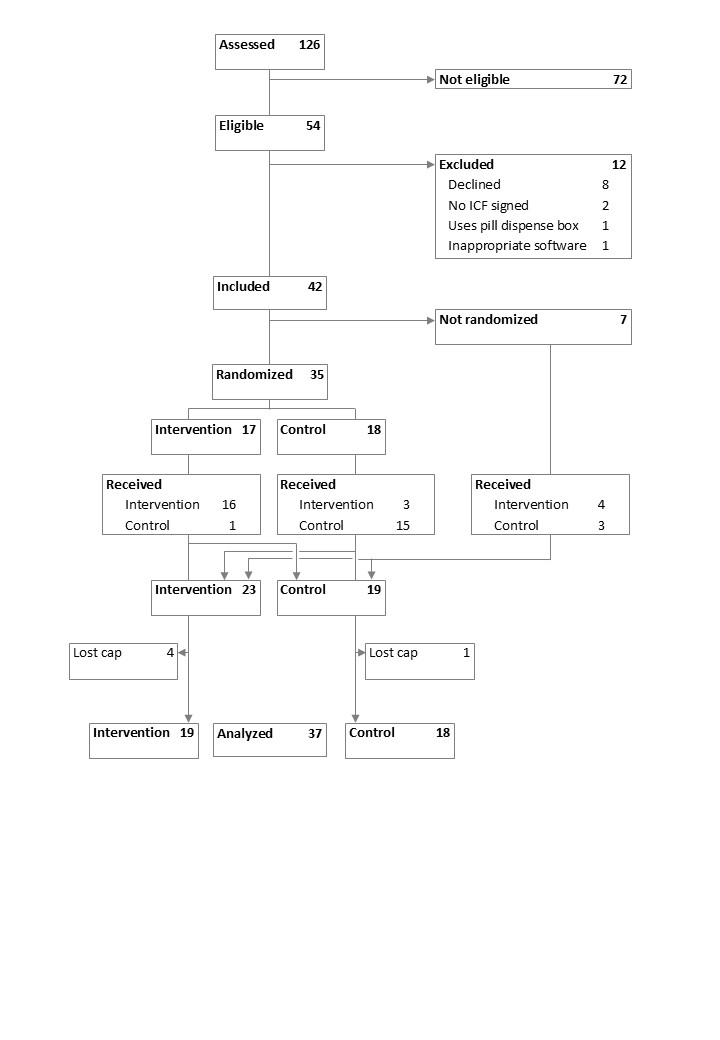
\includegraphics[width=.5\linewidth]{media/media/image1.jpg}
\caption{Flow diagram}
\end{figure}

\end{document}
